\documentclass{article}
\usepackage[utf8]{inputenc}
\usepackage[spanish]{babel}
\usepackage{listings}
\usepackage{graphicx}
\usepackage{geometry}
\graphicspath{ {images/} }
\usepackage{cite}

\geometry{
textheight=23cm
}
\begin{document}

\begin{titlepage}
    \begin{center}
        \vspace*{0cm}
            
        \large
        \textbf{ARTIC WOLF: SAVING THE FAMILY}
            
        \vfill
            
        \vspace{0.8cm}
            
        \textbf{David Agudelo Ochoa}
        
        \vspace{5mm}
        
        \textbf{Erika Dayana León Quiroga}
            
        \vfill
            
        \vspace{0.8cm}
            
        \Large
        Universidad de Antioquia\\
        Despartamento de Ingeniería Electrónica y Telecomunicaciones\\
        Informática II\\
        Medellín-Antioquia\\
        Abril de 2021
            
    \end{center}
\end{titlepage}

\tableofcontents
\newpage
\section{Sección introductoria.}
En este informe veremos el desarrollo del proyecto final de la materia Informática II, el cual será un juego llamado Gartic Wolf: Saving the family. Dentro de las secciones veremos listas de tareas hechas para organizar mejor el trabajo a realizar, actualizaciones y problemas del código del programa.

\section{Lista de tareas.}
\begin{itemize}
    \item Jueves 7 de Abril:
    \begin{itemize}
        \item Crear proyecto Qt
        \item Crear la clase ObjetoAnimado y las que heredarán de ella.
        \item Objeto animado: Atributos y métodos.
        \item Método StringPath.
        \item Probar método animar.
        \item Instalar librería QMediaPlayer (para sonidos del juego.)
        
    \end{itemize}
    \item Viernes 8 de Abril:
    \begin{itemize}
        \item Agregar atributos y constructor de las clases que heredan de Objeto animado, como héroe, enemigo, proyectil, reloj.
        \item Creación y animación del escenario y el héroe.
        \item Pruebas de la animación.
    
    \end{itemize}
    
    \item Sábado 9 de Abril:
    \begin{itemize}
        \item Agregar métodos de las clases que heredan de Objeto animado, como héroe, enemigo, proyectil, reloj.
        \item Método de proyectil que mueve y verifica la colisión con otros objetos del mismo.
        \item Agregar el método que creará el nivel uno.
    \end{itemize}
    
    \item Domingo 10 de Abril:
    \begin{itemize}
        \item Buscar ecuaciones de péndulo.
        \item Conectar las vidas, y el tiempo con la finalización del nivel.
        \item Agregar el menú.
        \item Personalizar el menú.
    \end{itemize}
    
    \item Lunes 11 de Abril:
    \begin{itemize}
        \item Modelar el comportamiento del péndulo.
        \item Terminar nivel uno.
        
        \item Tareas faltantes:
        \begin{itemize}
            \item Asignar botones de comandos.
            \item Diseñar la imagen del menú con los comandos previamente establecidos.
            \item Diseñar pantallas de información, como las intrucciones, la historia. Y pantallas de carga como el cambio de nivel.
            \item Implementar el poder del héroe.
        \end{itemize}
    \end{itemize}
    
    \item Martes 12 de Abril:
    \begin{itemize}
        \item Empezar a trabajar en el guardado del juego.
        \item Ecuaciones para el resorte y el movimiento parabólico.
        \item Modelar proyectil de nivel dos.
    \end{itemize}
    
    \item Miércoles 13 de Abril:
    \begin{itemize}
        \item Agregar movimiento del jugador en el nivel dos.
        \item Prueba de la jugabilidad del nivel dos.
        \item Estructuración de las pantallas de carga e información.
    \end{itemize}
    
    \item Jueves 14 de Abril:
    \begin{itemize}
        \item Diseño de las pantallas de información y carga.
    \end{itemize}
    
    
\end{itemize}

\section{Desarrollo del proyecto.}
Para el desarrollo del proyecto Artic Wolf: Saving the Family, se tuvo en cuenta el informe de Clases que se realizó previamente con la intención de tener un plan de organización de las clases que serían necesarias para el funcionamiento del juego que se tiene planeado. En este informe de clases encontramos la descripción nivel por nivel del juego y la descripción clase por clase del mismo. A continuación veremos los cambios que se le realizaron a las clases que se tenían pensadas a la hora de materializar estas ideas en código.

\subsection{Jueves 7 y Viernes 8 de Abril.}

Se comenzó por crear el proyecto con la clase padre Objeto animado con sus respectivos atributos y métodos, y sus clases hijas Heroe, Enemigo, Proyectil y Reloj.
En la clase objeto animado se realizaron varios cambios con respecto a lo planeado en el informe de clases. Esto porque a medida que se va escribiendo el código se encuentran formas más efectivas de realizar ciertas tareas que las que ya se tenían planeadas. Sin embargo, el uso del informe de Clases es fundamental para la asignación de tareas y la realización del avance del proyecto.

\begin{figure}[h]
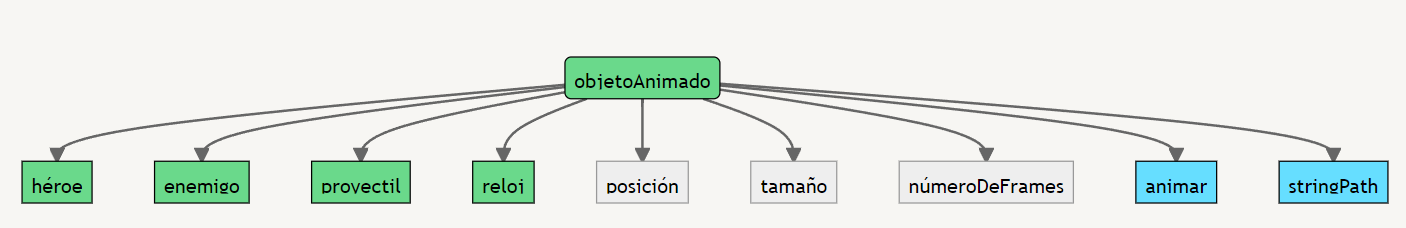
\includegraphics[scale=0.5]{Images/ObjetoAnimado.png}
\centering
\caption{Clase ObjetoAnimado que se tenía pensada construir.}
\label{fig:objetoAnimado}
\end{figure}

\begin{figure}[h]
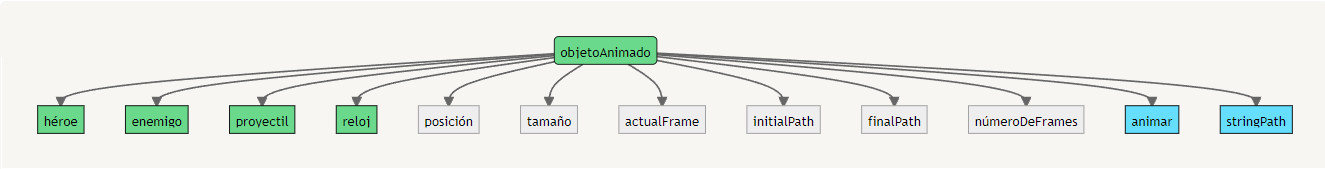
\includegraphics[scale=0.6]{Images/newObjetoanimado.png}
\centering
\caption{Clase ObjetoAnimado construida.}
\label{fig:newobjetoAnimado}
\end{figure}

Con los cambios realizados en la clase objeto animado se logró obtener el movimiento esperado en los objetos que se muestran en la escena, esto con ayuda del método animar y stringPath los cuales siguen cumpliendo las mismas funciones que se les asignaron en la parte de planeación del proyecto. El método stringPath recibe el número de la imagen de la cuál se requiere su path y luego lo retorna. La función animar utiliza el método anterior para conocer el camino a la imagen y haciendo uso de actualFrame como parámetro del método stringPath logra ir cambiando el frame de tal forma que cuando sea llamada, estos varíen y den la impresión de movimiento.

\newpage
\begin{figure}[h]
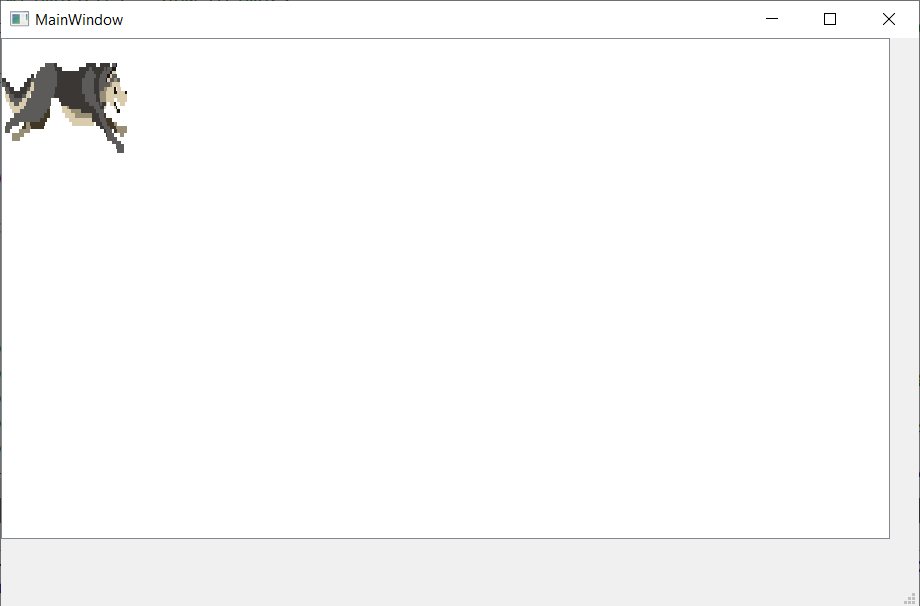
\includegraphics[scale=0.6]{Images/animacionInicial.png}
\centering
\caption{Pruebas del funcionamiento de la clase objeto animado.}
\label{fig:animacion1}
\end{figure}

\begin{figure}[h]
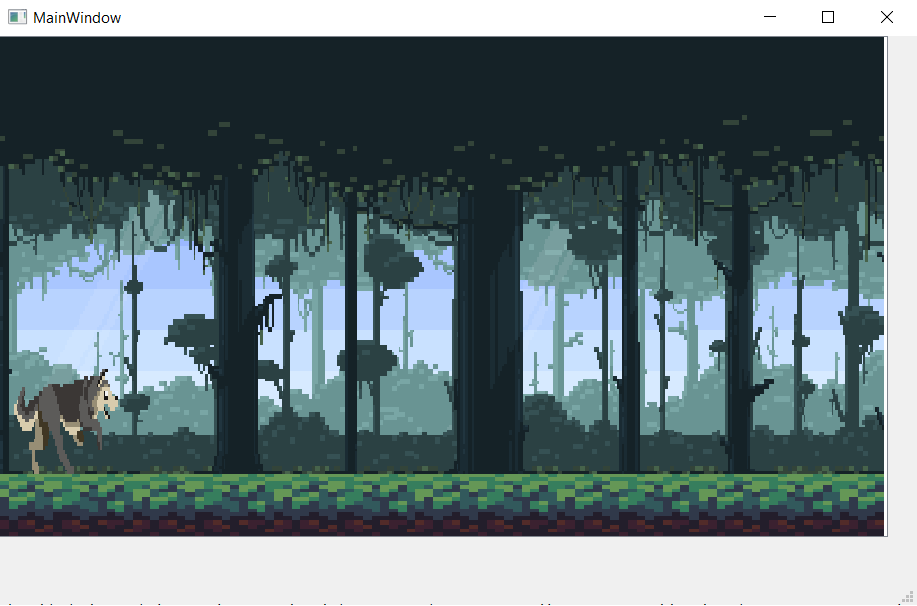
\includegraphics[scale=0.6]{Images/animaciones.png}
\centering
\caption{Pantalla de prueba con el héroe y el fondo animados.}
\label{fig:animacion}
\end{figure}

\subsection{Sábado 9 de Abril.}
Se empezó con la creación de la clase padre Nivel y sus clases hijas nivel1 y nivel2 como se planeó en el informe de Clases. Estas clases se utilizarían para armar el nivel correspondiente en cada clase.

\newpage
\begin{figure}[h]
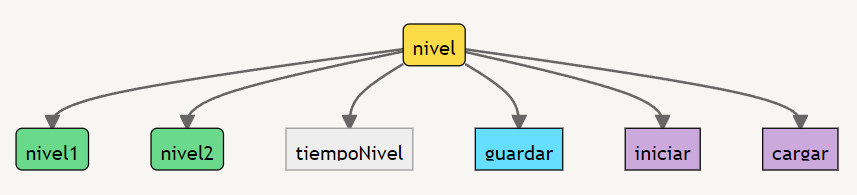
\includegraphics[scale=0.6]{Images/niveles.png}
\centering
\caption{Clase nivel planeada en el informe de clases.}
\label{fig:niveles}
\end{figure}

Sin embargo, nos dimos cuenta que la función que le otorgamos a estas clases en la planeación podría ser reemplazada por un \textbf{método en el MainWindow} que realice la misma función, en este método se agregarían todos los objetos necesarios para crear el nivel correspondiente. Por lo tanto la clase padre nivel y sus hijas son descartadas.

Este mismo día se comienza con el modelamiento del proyectil del nivel 1, para esto utilizamos el planteamiento de la clase proyectil que se realizó en el informe de clases.

\begin{figure}[h]
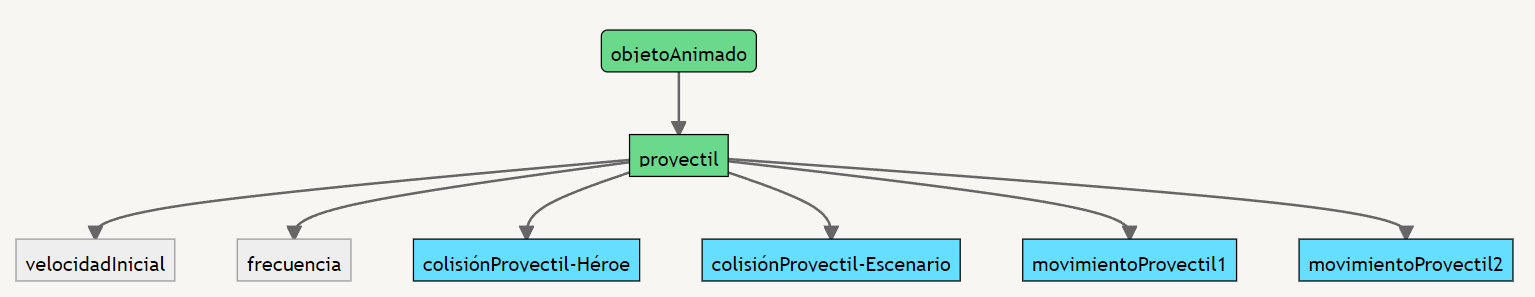
\includegraphics[scale=0.5]{Images/proyectil.png}
\centering
\caption{Clase nivel planeada en el informe de clases.}
\label{fig:proyectil}
\end{figure}

Se trabaja en la colisión entre el proyectil y el escenario, tratando de que cada que el proyectil salga de este se borre de la escena y se cree un nuevo proyectil, pero el borrado de este objeto provocaba conflictos en el proyecto por lo que se decidió que no se borraría el objeto sino que se le haría una especie de Reset a su posición, de esta forma no se estarían creando y borrando nuevos objetos sino que siempre es el mismo, y cuando sale de la escena o se choca con el héroe vuelve a su posición inicial.
El movimiento automático del proyectil se logra haciendo uso de un Timer y conectándolo con las ecuaciones de movimiento del proyectil del nivel 1.

\begin{figure}[h]
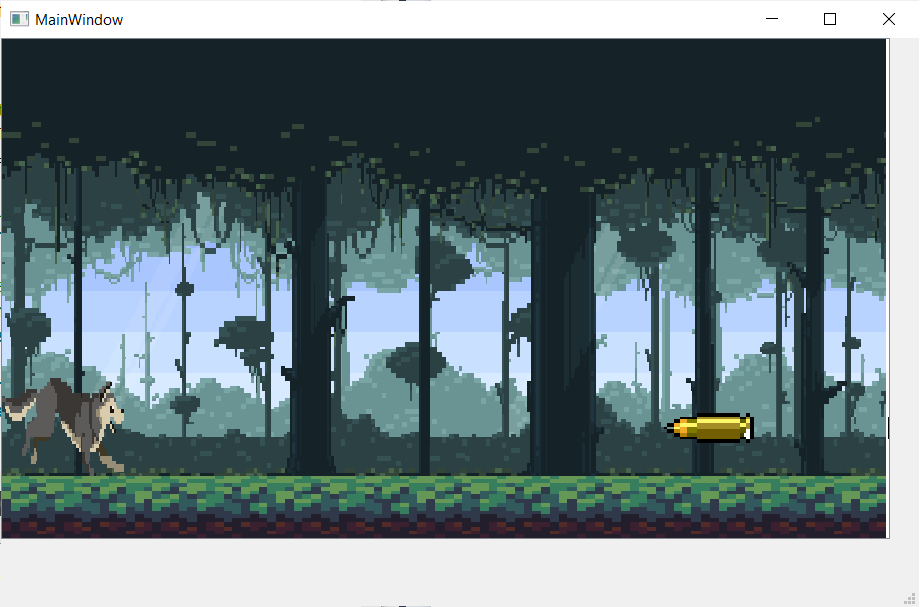
\includegraphics[scale=0.55]{Images/proyectil1.png}
\centering
\caption{Pruebas de la animación y la colisión entre el proyectil y la pared.}
\label{fig:proyectil1}
\end{figure}

\begin{figure}[h]
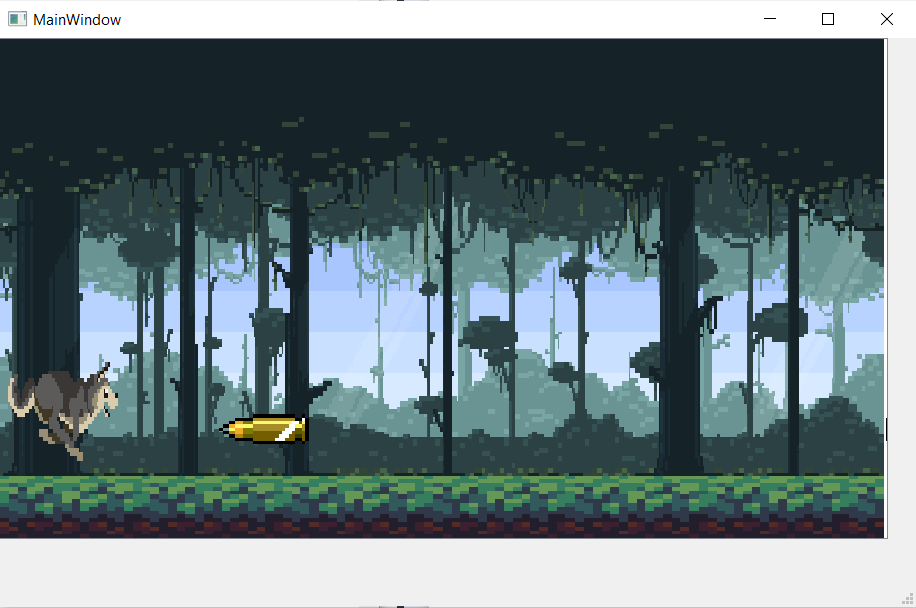
\includegraphics[scale=0.55]{Images/proyectil2.png}
\centering
\caption{Pruebas de la animación y la colisión entre el proyectil y la pared.}
\label{fig:proyectil2}
\end{figure}

\subsection{Domingo 10 de Abril.}
Se agregó la animación del enemigo, se ajustó la ventana de GraphicsView y el tamaño de todos los objetos en la escena.

\begin{figure}[h]
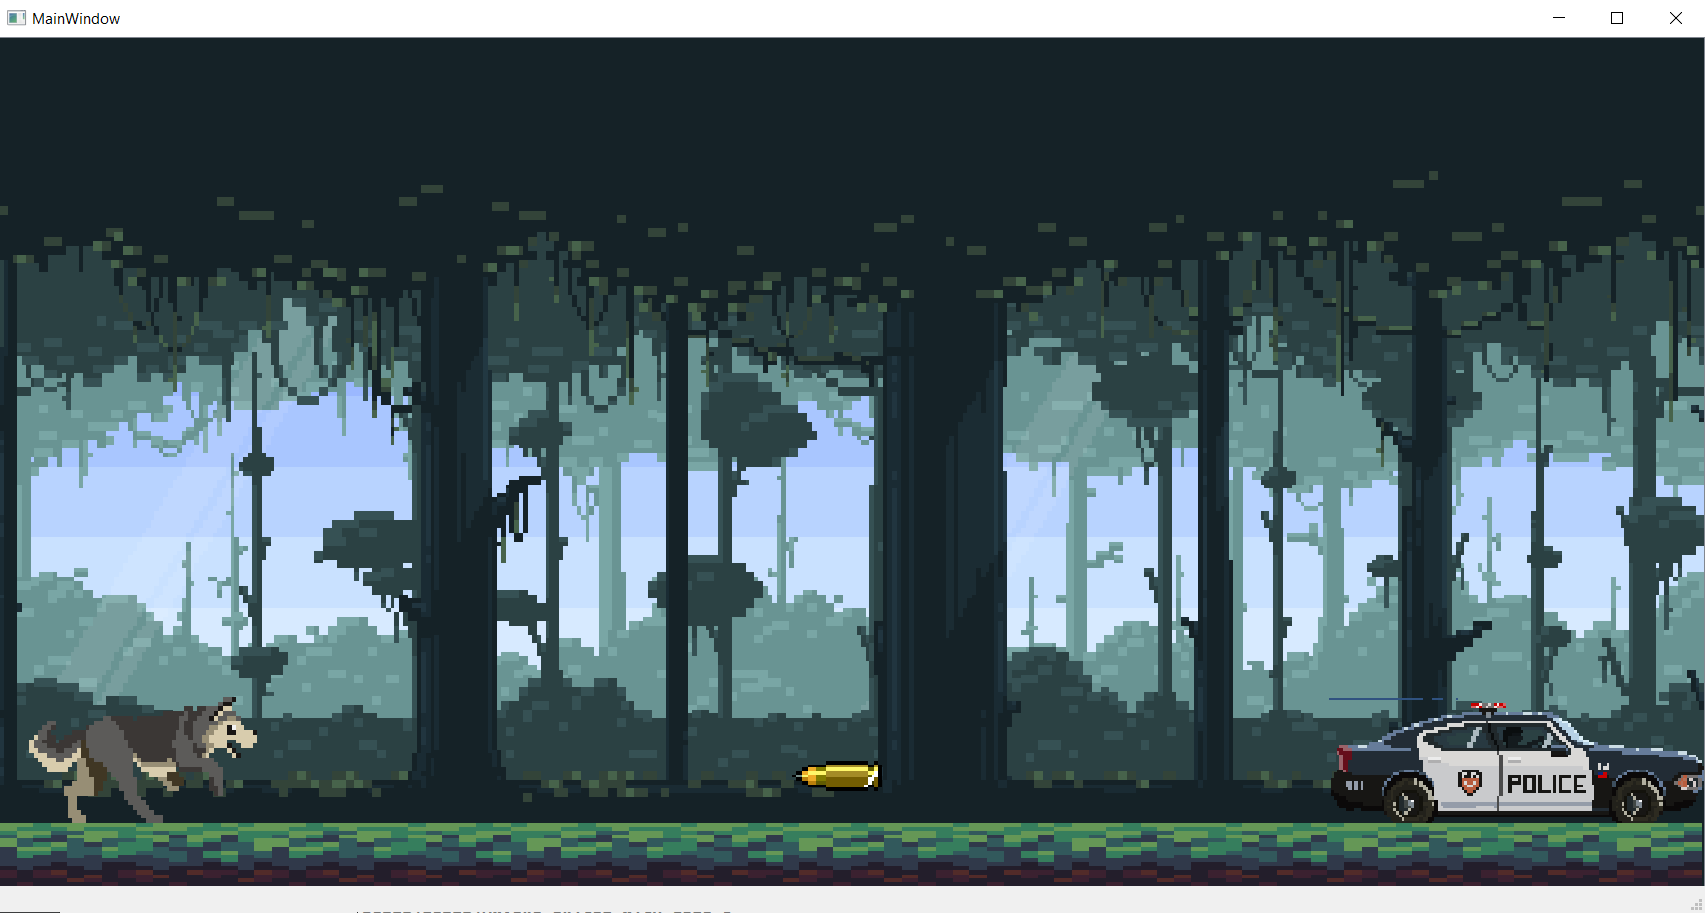
\includegraphics[scale=0.3]{Images/tamaniobjetosajustado.png}
\centering
\caption{Ajuste del tamaño de los objetos de la escena.}
\label{fig:ajustetamanio}
\end{figure}

También se agregó el contador de las vidas y del tiempo de la partida como podremos ver en la siguiente imagen (\ref{fig:vidastiempo}), estos contadores se ubicarán en la parte superior izquierda de la escena, en la imagen de demostración están encerrados en un recuadro rojo para ubicarlos de la manera más sencilla. El tiempo irá disminuyendo conforme transcurre la partida con ayuda de un Timer. Las vidas disminuirán cada que un proyectil choque con el héroe y esto será codificado en el método de la clase proyectil en donde se verifica la colisión entre el héroe y el proyectil.

\newpage
\begin{figure}[h]
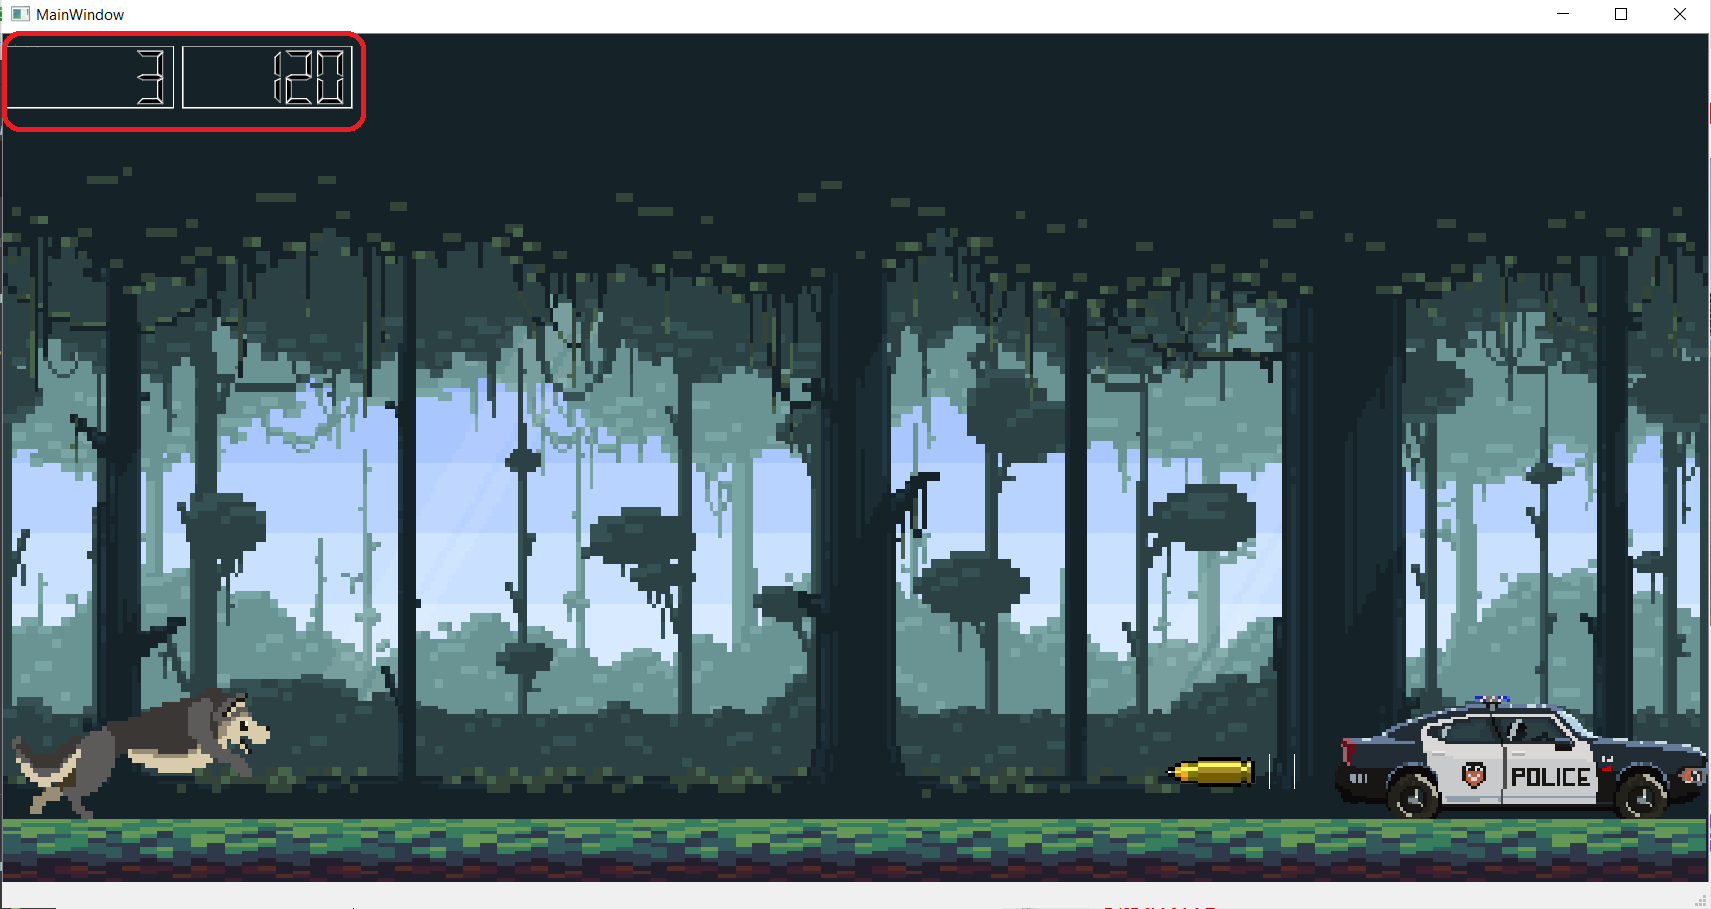
\includegraphics[scale=0.4]{Images/tiempovidas.png}
\centering
\caption{Reloj y vidas del héroe puestas en pantalla.}
\label{fig:vidastiempo}
\end{figure}

Se hicieron pruebas para agregar la pantalla del menú, la cuál aparecerá cuando se corra el juego y una vez se presione la tecla I del teclado iniciará la partida con tres vidas y 120 segundos en el contador del tiempo de la partida. Esto se hará con un KeyPressEvent y un if que al presionar la tecla determinada iniciará el método del MainWindow encargado de crear los objetos del nivel 1.

\begin{figure}[h]
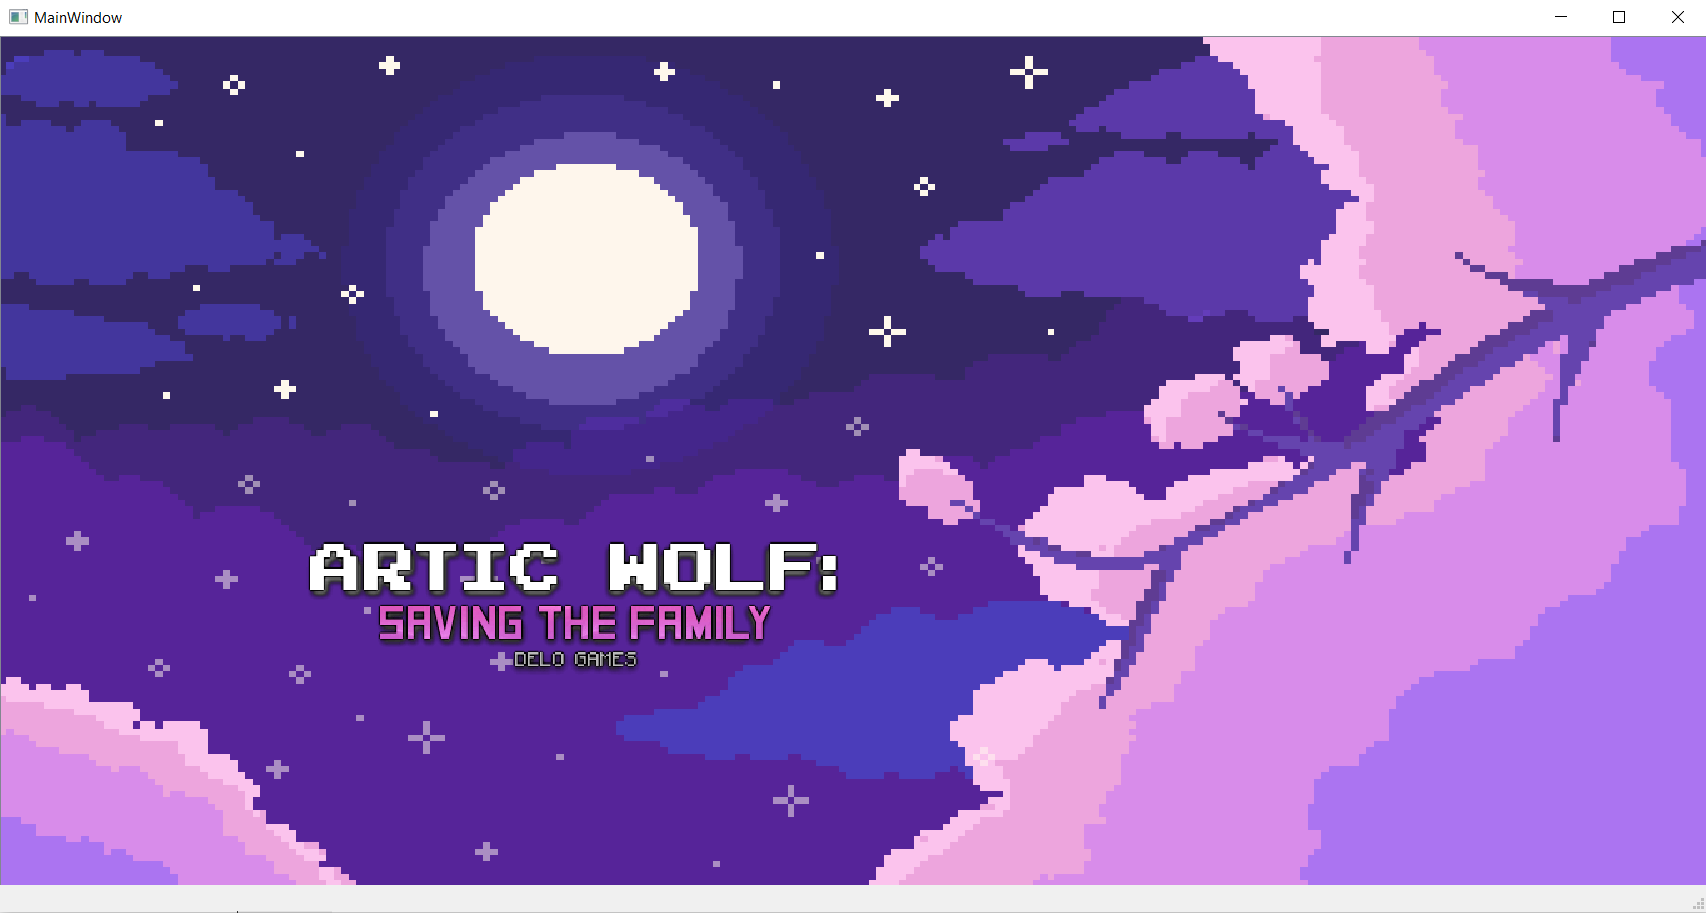
\includegraphics[scale=0.4]{Images/pantallainicio.png}
\centering
\caption{Pantalla que mostrará el menú.}
\label{fig:pantallamenu}
\end{figure}

\newpage
\begin{figure}[h]
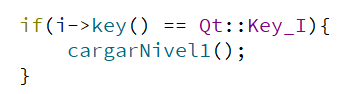
\includegraphics[scale=1]{Images/keyi.png}
\centering
\caption{Condicional encargado de iniciar el nivel 1 cuando se presione la tecla I.}
\label{fig:if}
\end{figure}

 \textbf{PROBLEMAS:} La animación del héroe tiene problemas en el momento en el que el héroe se encuentra realizando un salto. Esto se debe a que la animación del enemigo se encuentra dentro del SLOT de animación del héroe para ahorrar líneas de código.
 \newline
 \textbf{POSIBLES SOLUCIONES: }Una de las posibles soluciones es meter la animación del enemigo dentro de otro SLOT de animación que ya exista, como el del fondo o el proyectil para de esta forma seguir ahorrando líneas de código. La otra opción es simplemente crear un nuevo SLOT que se encargue de la animación del enemigo.
 \newline
 
\subsection{Lunes 11 de Abril.}
Se comenzó solucionando el problema que se venía presentando con la animación del enemigo, se probaron las dos posibles soluciones planteadas y se tomó la decisión de crear un nuevo SLOT para la animación del enemigo así esto conllevara líneas extras de código. Luego de que el problema anterior fue solucionado se procedió a realizar el modelamiento del péndulo y la descripción de este movimiento con ayuda de un diagrama de cuerpo libre y las ecuaciones. 

\begin{figure}[h]
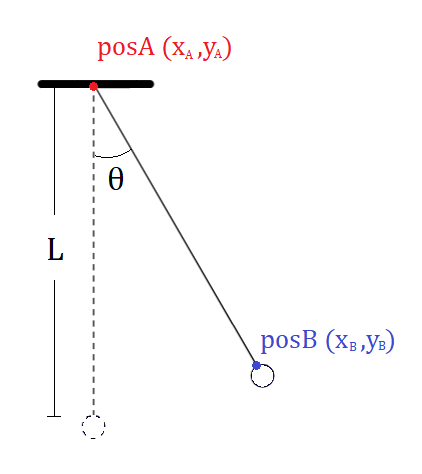
\includegraphics[scale=0.6]{Images/diagramapendulo.png}
\centering
\caption{Diagrama de cuerpo libre del péndulo.}
\label{fig:diagrama}
\end{figure}

Para esto se agregaron nuevos atributos a la clase del reloj, como la longitud del péndulo, sus coordenadas en los puntos A y B y el ángulo inicial del mismo.

\begin{figure}[h]
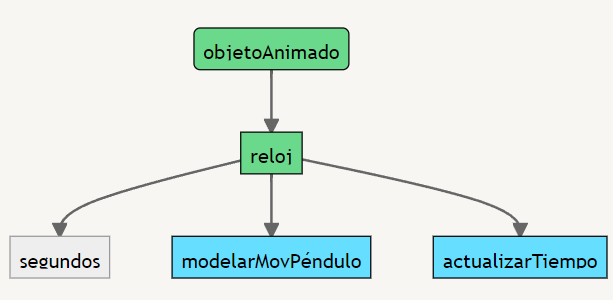
\includegraphics[scale=0.5]{Images/reloj.png}
\centering
\caption{Clase reloj pensada en el informe de Clases.}
\label{fig:reloj}
\end{figure}

\begin{figure}[h]
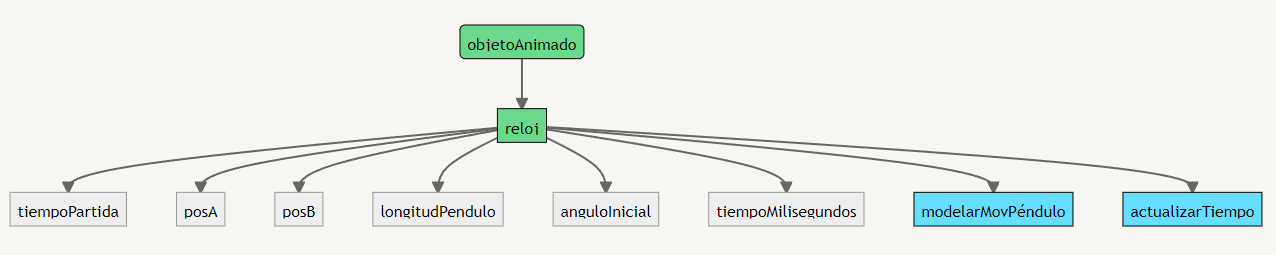
\includegraphics[scale=0.6]{Images/newreloj.png}
\centering
\caption{Clase reloj necesaria para la creación del péndulo.}
\label{fig:newreloj}
\end{figure}

También se creó un constructor diferente para el reloj, en el que se incluyen los valores iniciales necesarios para la construcción del péndulo, estos valores serán las coordenadas del punto A, la longitud del péndulo y el ángulo inicial y con los valores anteriormente mencionados se obtendrán las coordenadas iniciales del punto B. Esto, como ya se mencionó, serán los valores de las coordenadas iniciales del péndulo.

\begin{figure}[h]
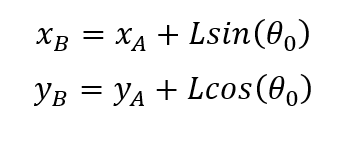
\includegraphics[scale=0.6]{Images/ecuacion1.png}
\centering
\caption{Ecuaciones para determinar las coordenadas iniciales del punto B.}
\label{fig:ecu2}
\end{figure}

Luego, para realizar el movimiento pendular se necesitará ir cambiando las coordenadas en B con respecto avance el tiempo, para esto se necesitará el ángulo, que también irá cambiando con respecto al tiempo, un omega que está relacionado con la longitud del péndulo, la longitud del péndulo y las coordenadas en A.

\begin{figure}[h]
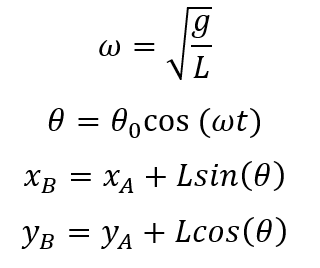
\includegraphics[scale=0.6]{Images/ecuacion2.png}
\centering
\caption{Ecuaciones que determinan el movimiento del péndulo. Siendo g la gravedad, L la longitud del péndulo, y theta sub cero el ángulo inicial.}
\label{fig:ecu1}
\end{figure}

Después de realizar la implementación de las ecuaciones del péndulo y verificar su funcionamiento, se agregó la imagen del reloj y del péndulo para la ambientación del juego.

\newpage
\begin{figure}[h]
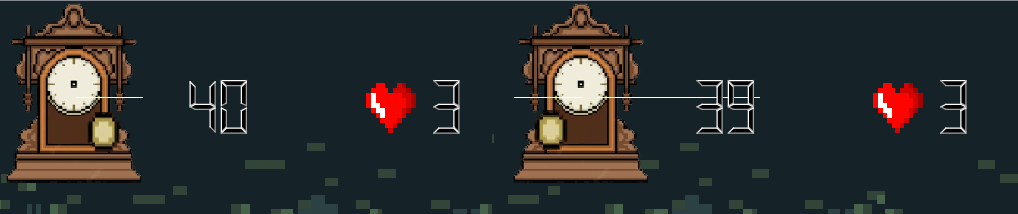
\includegraphics[scale=0.7]{Images/barra.png}
\centering
\caption{Imagen del reloj y péndulo funcionando.}
\label{fig:penduloreloj}
\end{figure}

Este mismo día se comenzó con la prueba de las ecuaciones de movimiento parabólico que serán utilizadas en el nivel 2 para el lanzamiento del proyectil.

\subsection{Martes 13 de Abril.}
Como se tenía planeado se comenzó a abordar el problema del guardado y la carga del juego, para comenzar se tendrán en cuenta los aspectos más importantes del juego, como lo son el número de vidas del héroe, el tiempo que lleva la partida y el nivel en el que se encuentra a la hora de guardar. Para esto se creó una nueva clase que no estaba contemplada en la planeación de las clases, pues en esta planeación se tenía pensado incluir el guardado y cargado en la clase de niveles, clase que finalmente no fue implementada en el código, por esto se creó una clase que se encarga de guardar y cargar las partidas cuando el usuario así lo requiere.
Para implementar la clase se utilizó la práctica tres como guía del manejo de archivos, pues es utilizando estos que podremos guardar y cargar la partida.

Para guardar la partida creamos un método que tendrá como parámetros su nombre, y punteros a objetos de tipo reloj y de tipo héroe, lo anterior para poder utilizar los métodos Get del tiempo de partida, las vidas del héroe y el nivel en el que se encuentra, que son los datos relevantes del juego. Los datos anteriores se escribirán en el archivo haciendo un salto de línea en cada uno para su fácil lectura cuando se desee cargar el juego.
Para cargar la partida se codificará otro método con los mismos parámetros del método de guardado, con la diferencia que el archivo de este método será de lectura, para tomar los datos guardados en el archivo de escritura y cargar el nivel con estos datos.

\begin{figure}[h]
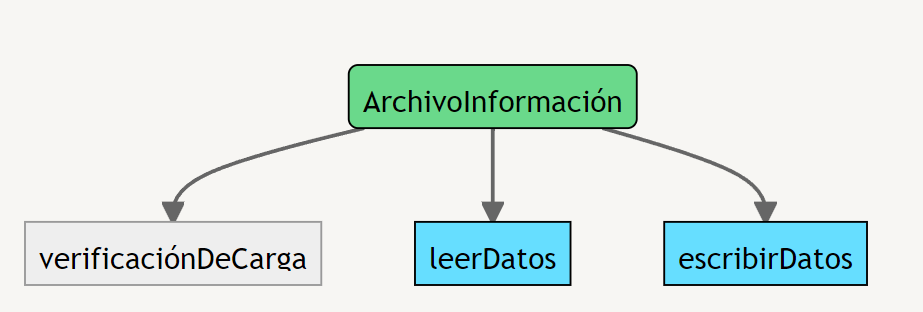
\includegraphics[scale=0.7]{Images/archivoinfo.png}
\centering
\caption{Mapa mental de la clase que manejará el guardado y cargado del juego.}
\label{fig:diagramaresorte}
\end{figure}

En este día también se implementó el Movimiento Parabólico haciendo uso de sus ecuaciones. Estas ecuaciones se utilizarán para el movimiento del proyectil del nivel dos.

\newpage
\begin{figure}[h]
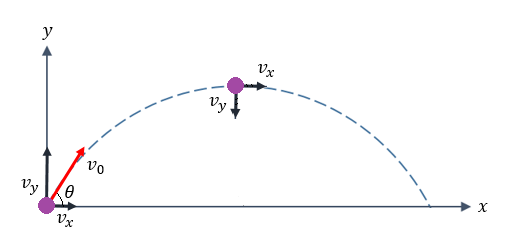
\includegraphics[scale=1]{Images/diagramaparabolico.png}
\centering
\caption{Diagrama de cuerpo libre del movimiento parabólico.}
\label{fig:diagramaresorte}
\end{figure}

\begin{figure}[h]
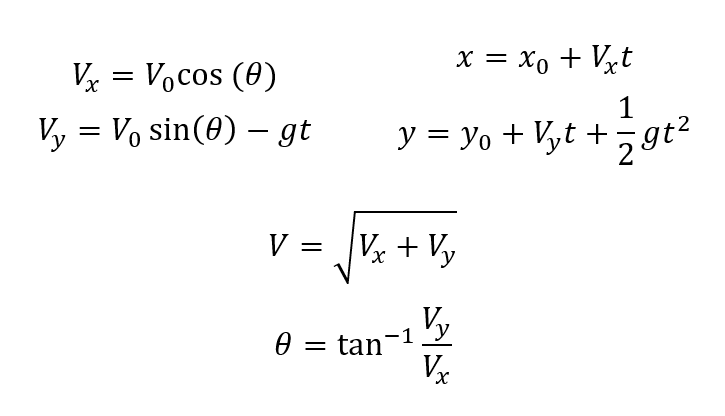
\includegraphics[scale=0.7]{Images/ecuacionparabolica.png}
\centering
\caption{Ecuaciones del movimiento parabólico.}
\label{fig:ecuacionesmovpara}
\end{figure}

También implementamos las ecuaciones de resortes, las cuales nos darán la velocidad inicial del proyectil que variará dependiendo de la compresión que se le realice al resorte, esta compresión será aleatoria. Para todas las ecuaciones usadas en este proyecto se tuvo que tener en cuenta el sistema de referencia de la escena en donde se agregan todos los objetos necesarios para el funcionamiento del juego.

\newpage
\begin{figure}[h]
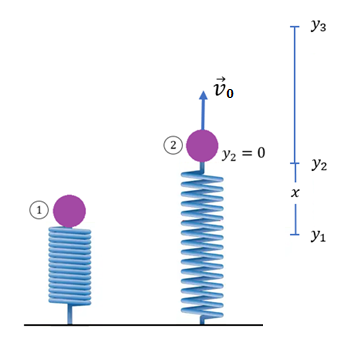
\includegraphics[scale=1]{Images/diagramaresorte.png}
\centering
\caption{Diagrama de cuerpo libre del resorte.}
\label{fig:diagramaresorte}
\end{figure}

\begin{figure}[h]
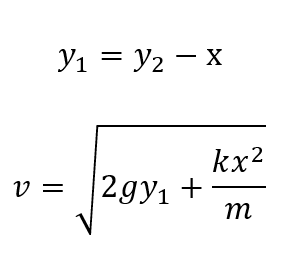
\includegraphics[scale=0.7]{Images/ecuacionresorte.png}
\centering
\caption{Ecuaciones para la velocidad inicial dada por un resorte.}
\label{fig:ecuacionesresorte}
\end{figure}

(IMAGEN DEL NIVEL DOS)

\subsection{Miércoles 13 y Jueves 14 de Abril.}
Este día se utilizó para agregarle más movilidad al héroe, movilidad que será vista como su poder dentro del juego, este poder será activado en especial para el nivel dos, pues es allí en donde se necesitará mover de izquierda a derecha y viceversa para esquivar los proyectiles que vienen con movimiento parabólico hacia el suelo y que pueden restarle vidas. Para el movimiento del héroe se utilizarán las teclas A (movimiento a la izquierda) y D (moviemiento a la derecha).

Se agregará una nueva animación para mostrar este poder, la cual se pondrá sobre la animación del héroe de forma que parezcan chispas saliendo de él.

(IMAGEN DEL HEROE Y SU PODER)

También se comenzó con la estructuración de las pantallas de información y de carga, pues la historia es una parte importante para comprender las dinámicas que veremos en el juego, también nos ayudarán a mostrar los controles de juego de cada nivel, de esta forma será más sencillo para el usuario recordar las opciones que tiene para controlar al héroe en cada nivel.

(DIAGRAMA DE FLUJO DE LAS PANTALLAS DE INFORMACIÓN Y CARGA)

Tendremos una pantalla de información y una pantalla de carga en cada nivel, la primera nos mostrará la historia del juego dependiendo del nivel y la segunda nos informará de los controles que debemos utilizar en cada nivel.

\begin{itemize}
    \item NIVEL 1.
    
        \begin{figure}[h]
        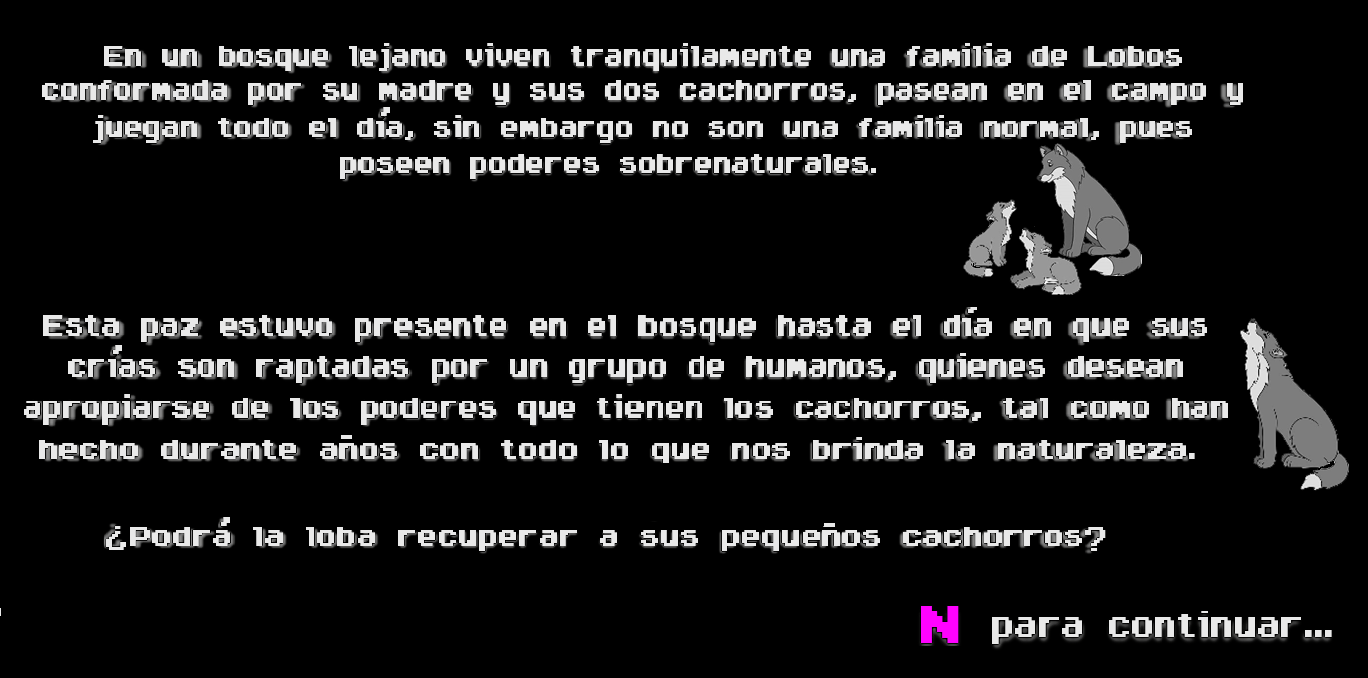
\includegraphics[scale=0.5]{Images/pantallahistoria.png}
        \centering
        \caption{Ecuaciones para la velocidad inicial dada por un resorte.}
        \label{fig:ecuacionesresorte}
        \end{figure}
    
    \item NIVEL 2.
        \begin{figure}[h]
        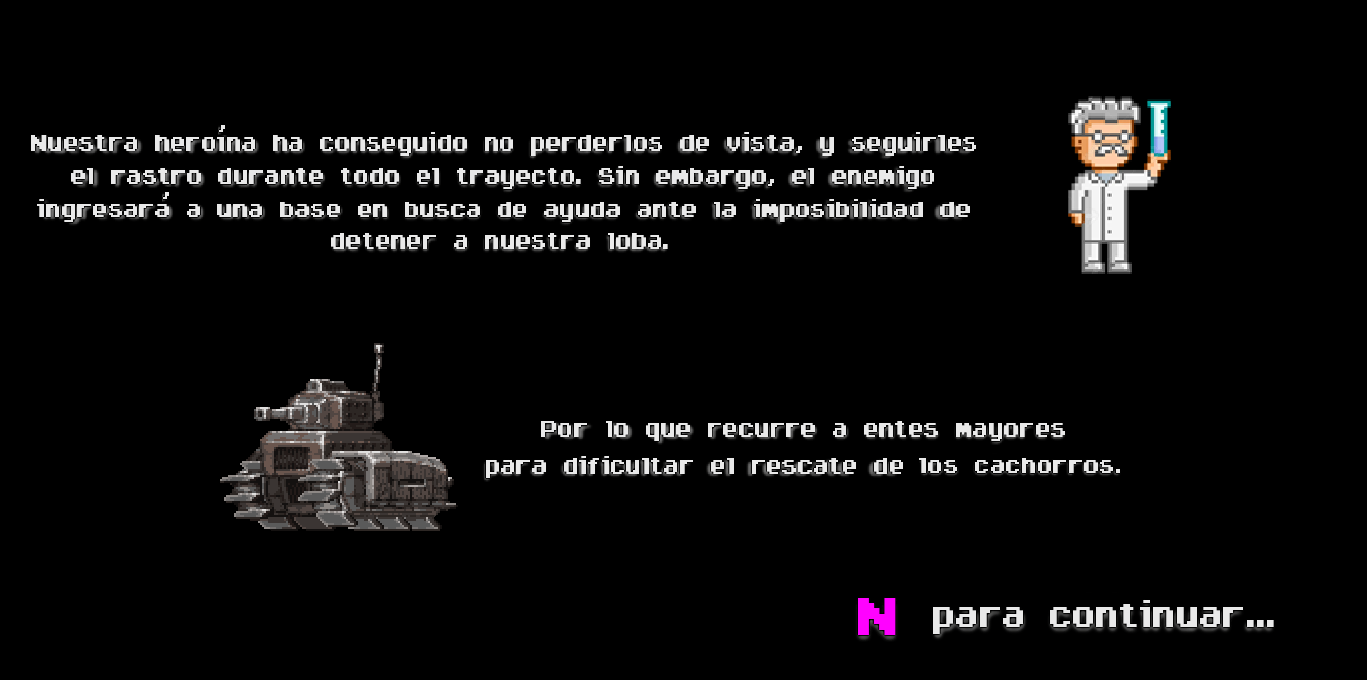
\includegraphics[scale=0.5]{Images/pantallahistoria2.png}
        \centering
        \caption{Ecuaciones para la velocidad inicial dada por un resorte.}
        \label{fig:ecuacionesresorte}
        \end{figure}
    
\end{itemize}




\section{Pantalla: Historia de Juego.}
MENU

En un bosque lejano viven tranquilamente una familia de Lobos conformada por su madre y sus dos cachorros, pasean en el campo y juegan todo el día, sin embargo no son una familia normal, pues poseen poderes sobrenaturales.

Esta paz estuvo presente en el bosque hasta el día en que sus crías son raptadas por un grupo de humanos, quienes desean apropiarse de los poderes que tienen los cachorros, tal como han hecho durante años con todo lo que nos brinda la naturaleza.

¿Podrá la loba recuperar a sus pequeños cachorros?

PANTALLA DE CARGA CON CONTROL W

NIVEL 1

Nuestra heroína ha conseguido no perderlos de vista, y seguirles el rastro durante todo el trayecto. Sin embargo, el enemigo ingresará a una base en busca de ayuda ante la imposibilidad de detener a nuestra loba.

Por lo que recurre a entes mayores para dificultar el rescate de los cachorros.




\end{document}
